\begin{frame}
\frametitle{Are terrorist relationships similar to social networks?}
If we find that relationships networks are similar to social networks then we could eventually understand how they form and how people join terrorist organisations.

\begin{itemize}
\item The relationships line graph is built from a graph. We can only get partial information about this original graph.
\item \emph{Transitivity} and \emph{homophily} are the main particularities of real social networks.
\item We found that some social networks are scale-free. 
\end{itemize}

\end{frame}

% ----------------------------------------------------------------------------------------

\begin{frame}
\frametitle{Making a scale free graph}

We build the line graph from a scale free graph with parameters that makes sense given the previously stated assumptions.

\begin{figure}[H]
\begin{center}
        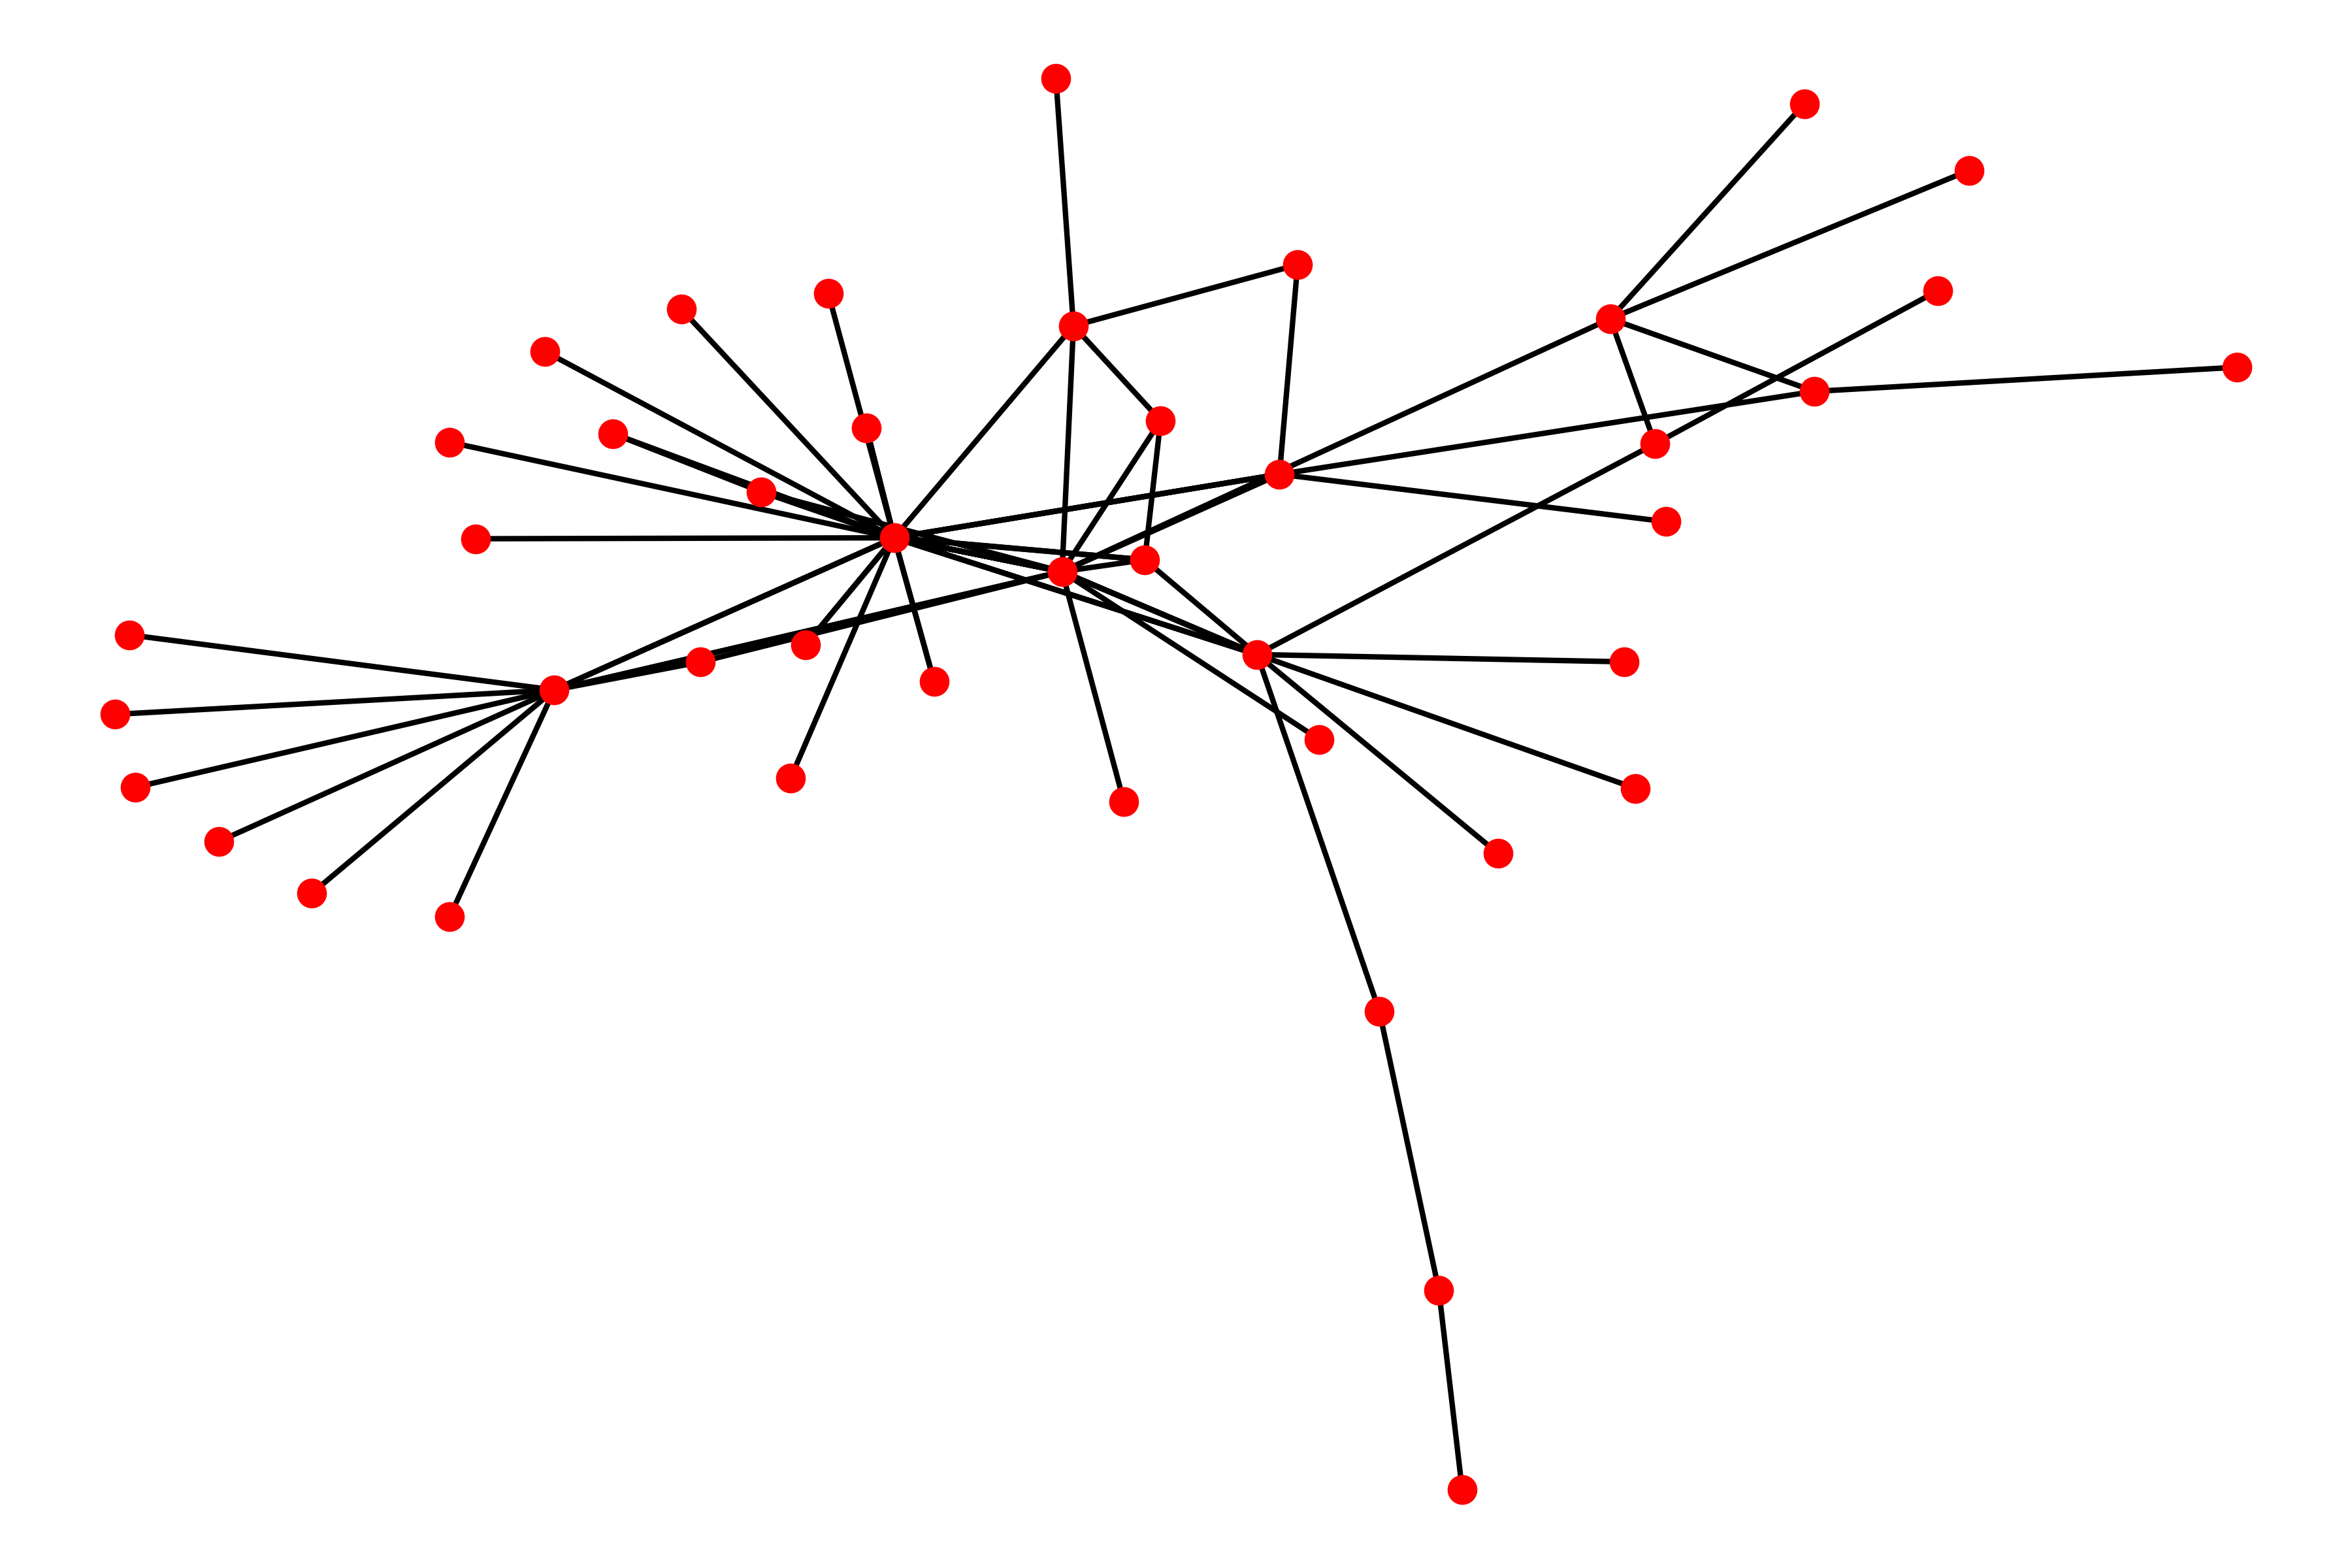
\includegraphics[width=0.5\textwidth]{graphScaleFree.png}
        \caption{Scale free network}
        \label{fig:Scalefree}
        \end{center}
\end{figure}
\end{frame}
    
% ----------------------------------------------------------------------------------------

\begin{frame}
\frametitle{Making a comparable line graph}
We make a line graph of the scale free network but can only compare it to one connected component, so we use the largest one of the dataset.

\begin{figure}[H]
\begin{center}
    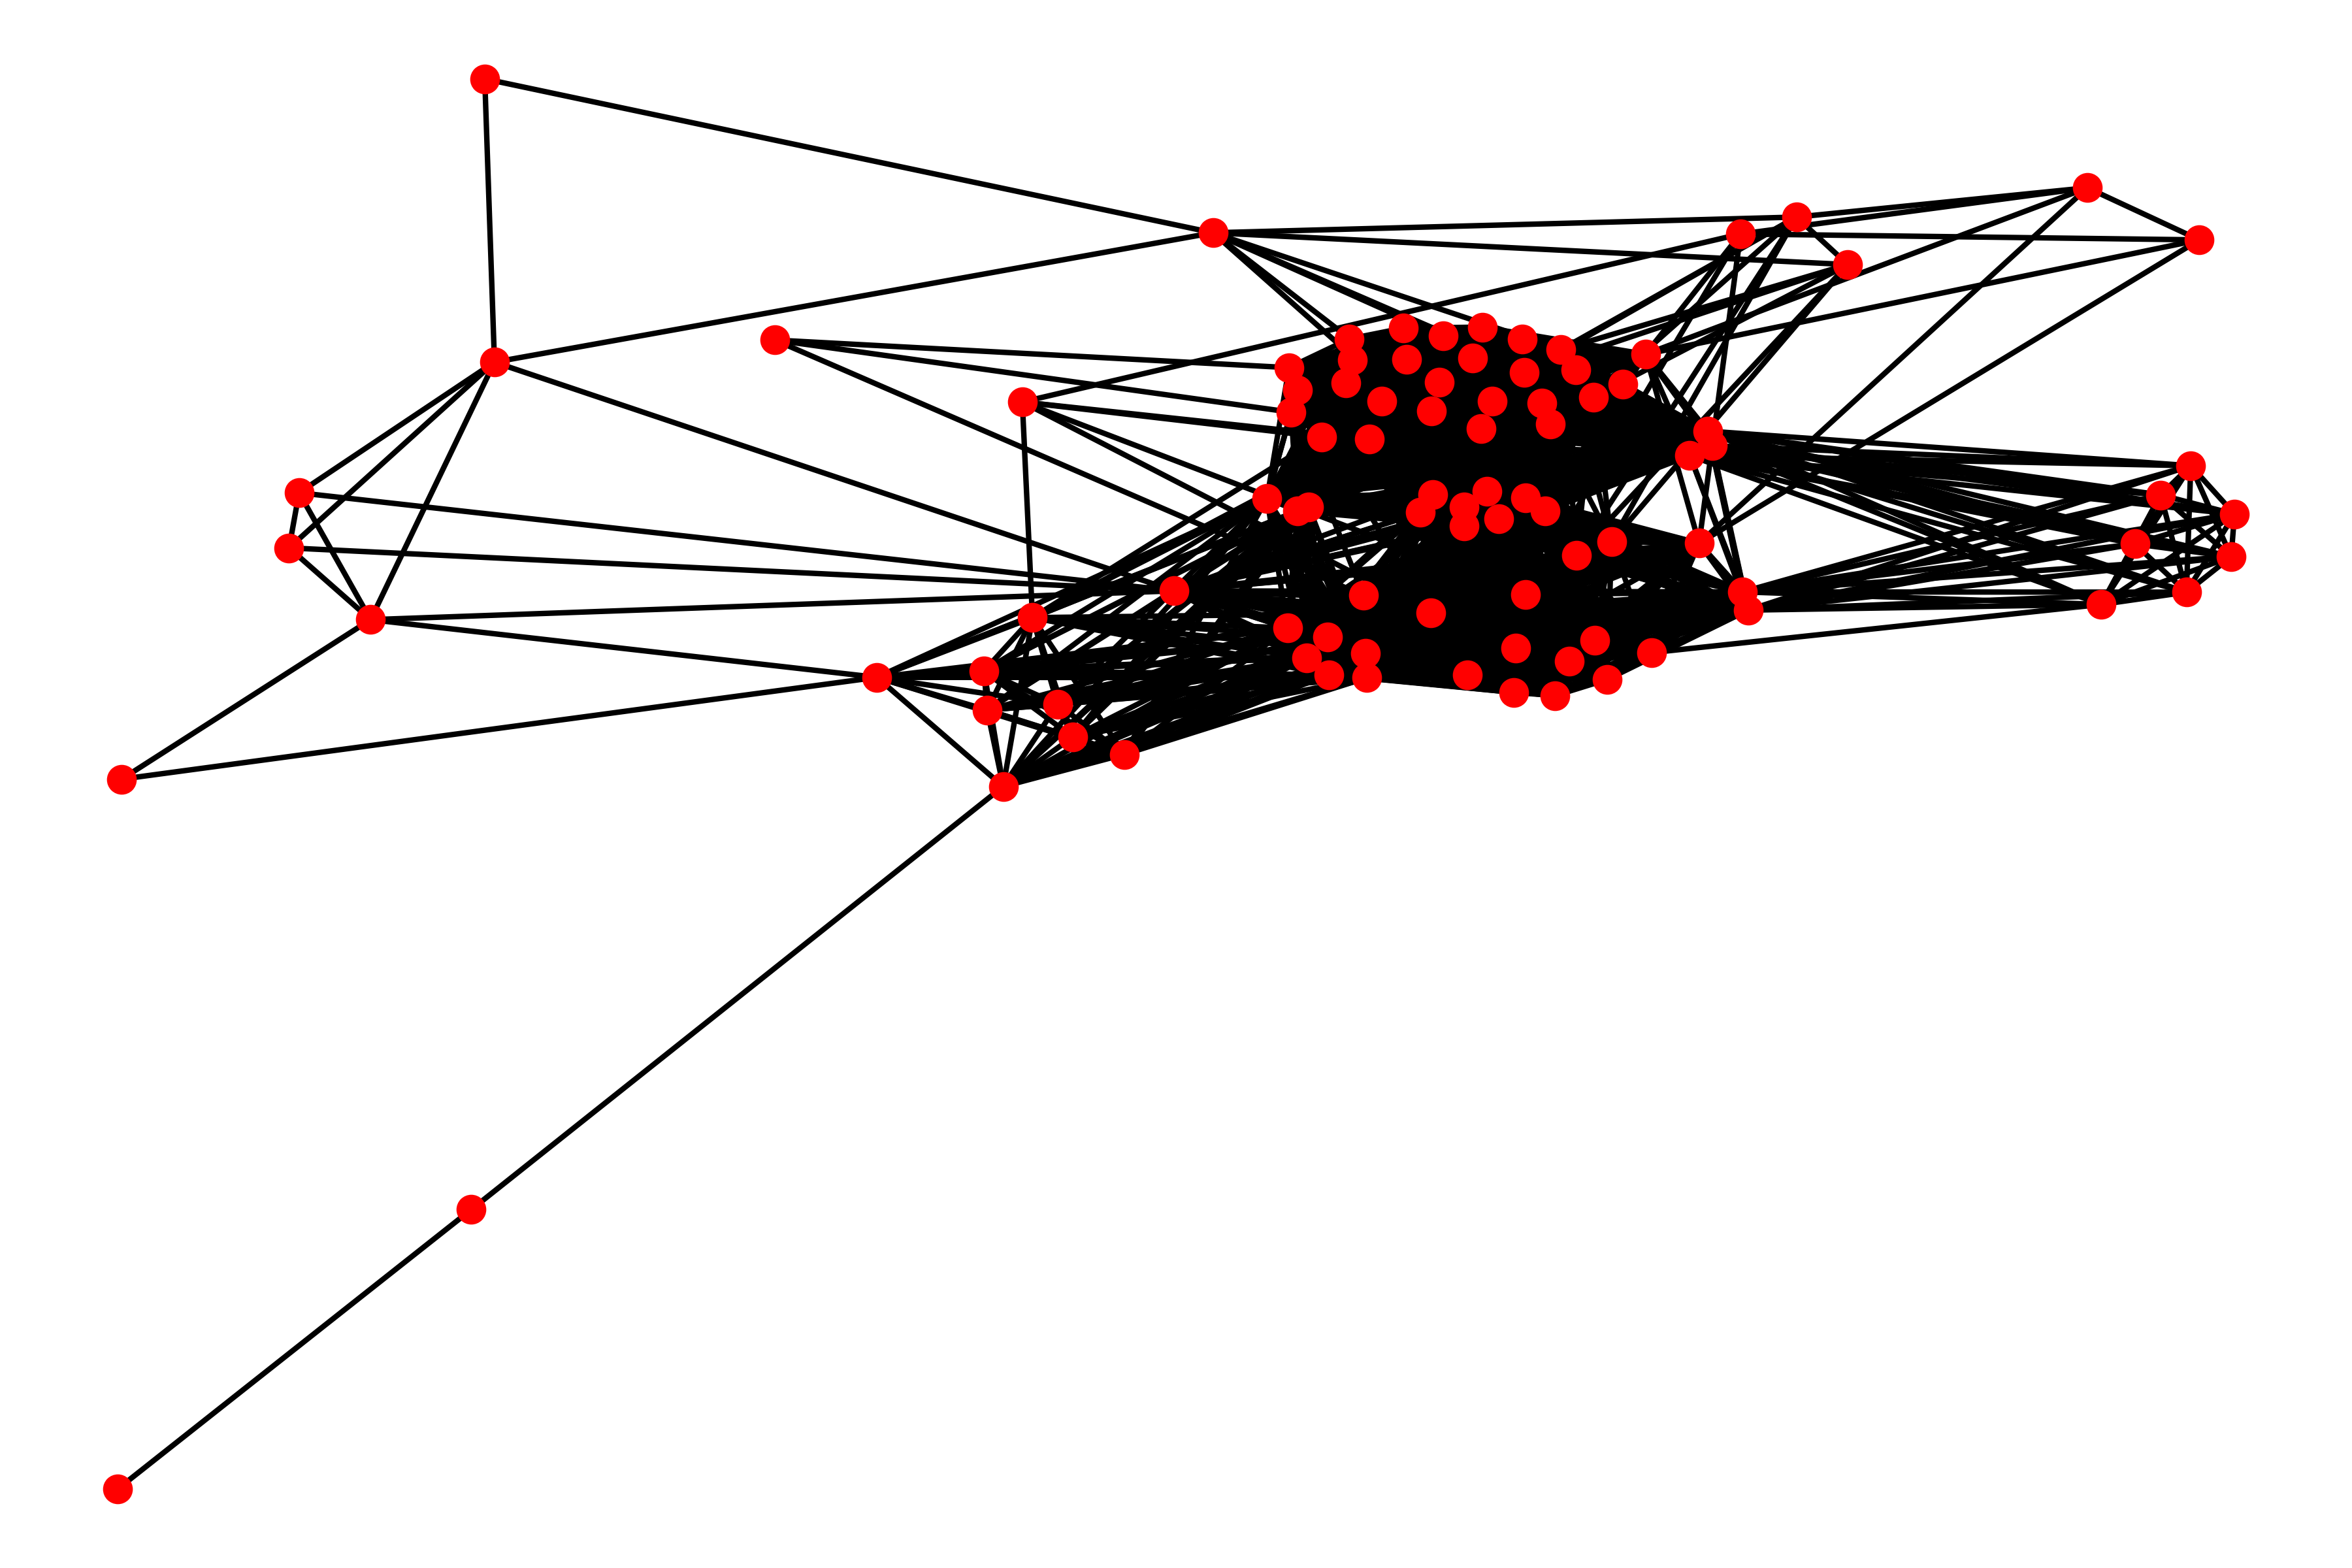
\includegraphics[width=0.5\textwidth]{graphLineScaleFree.png}
    \caption{Line graph of the scale free network}
    \label{fig:lineG}
\end{center}
\end{figure}
\end{frame}

% ----------------------------------------------------------------------------------------

\begin{frame}
\frametitle{Relationships dataset: Results}


Preliminary conclusion: The relationship network cannot be modeled by the line graph of a scale free network
\begin{itemize}
\item This could be because the relations of terrorist are not similar to social ties
\item The size of the largest component is too small, making it hard for a scale free graph to represent a social network.
\end{itemize}


\begin{figure}[H]
\begin{center}
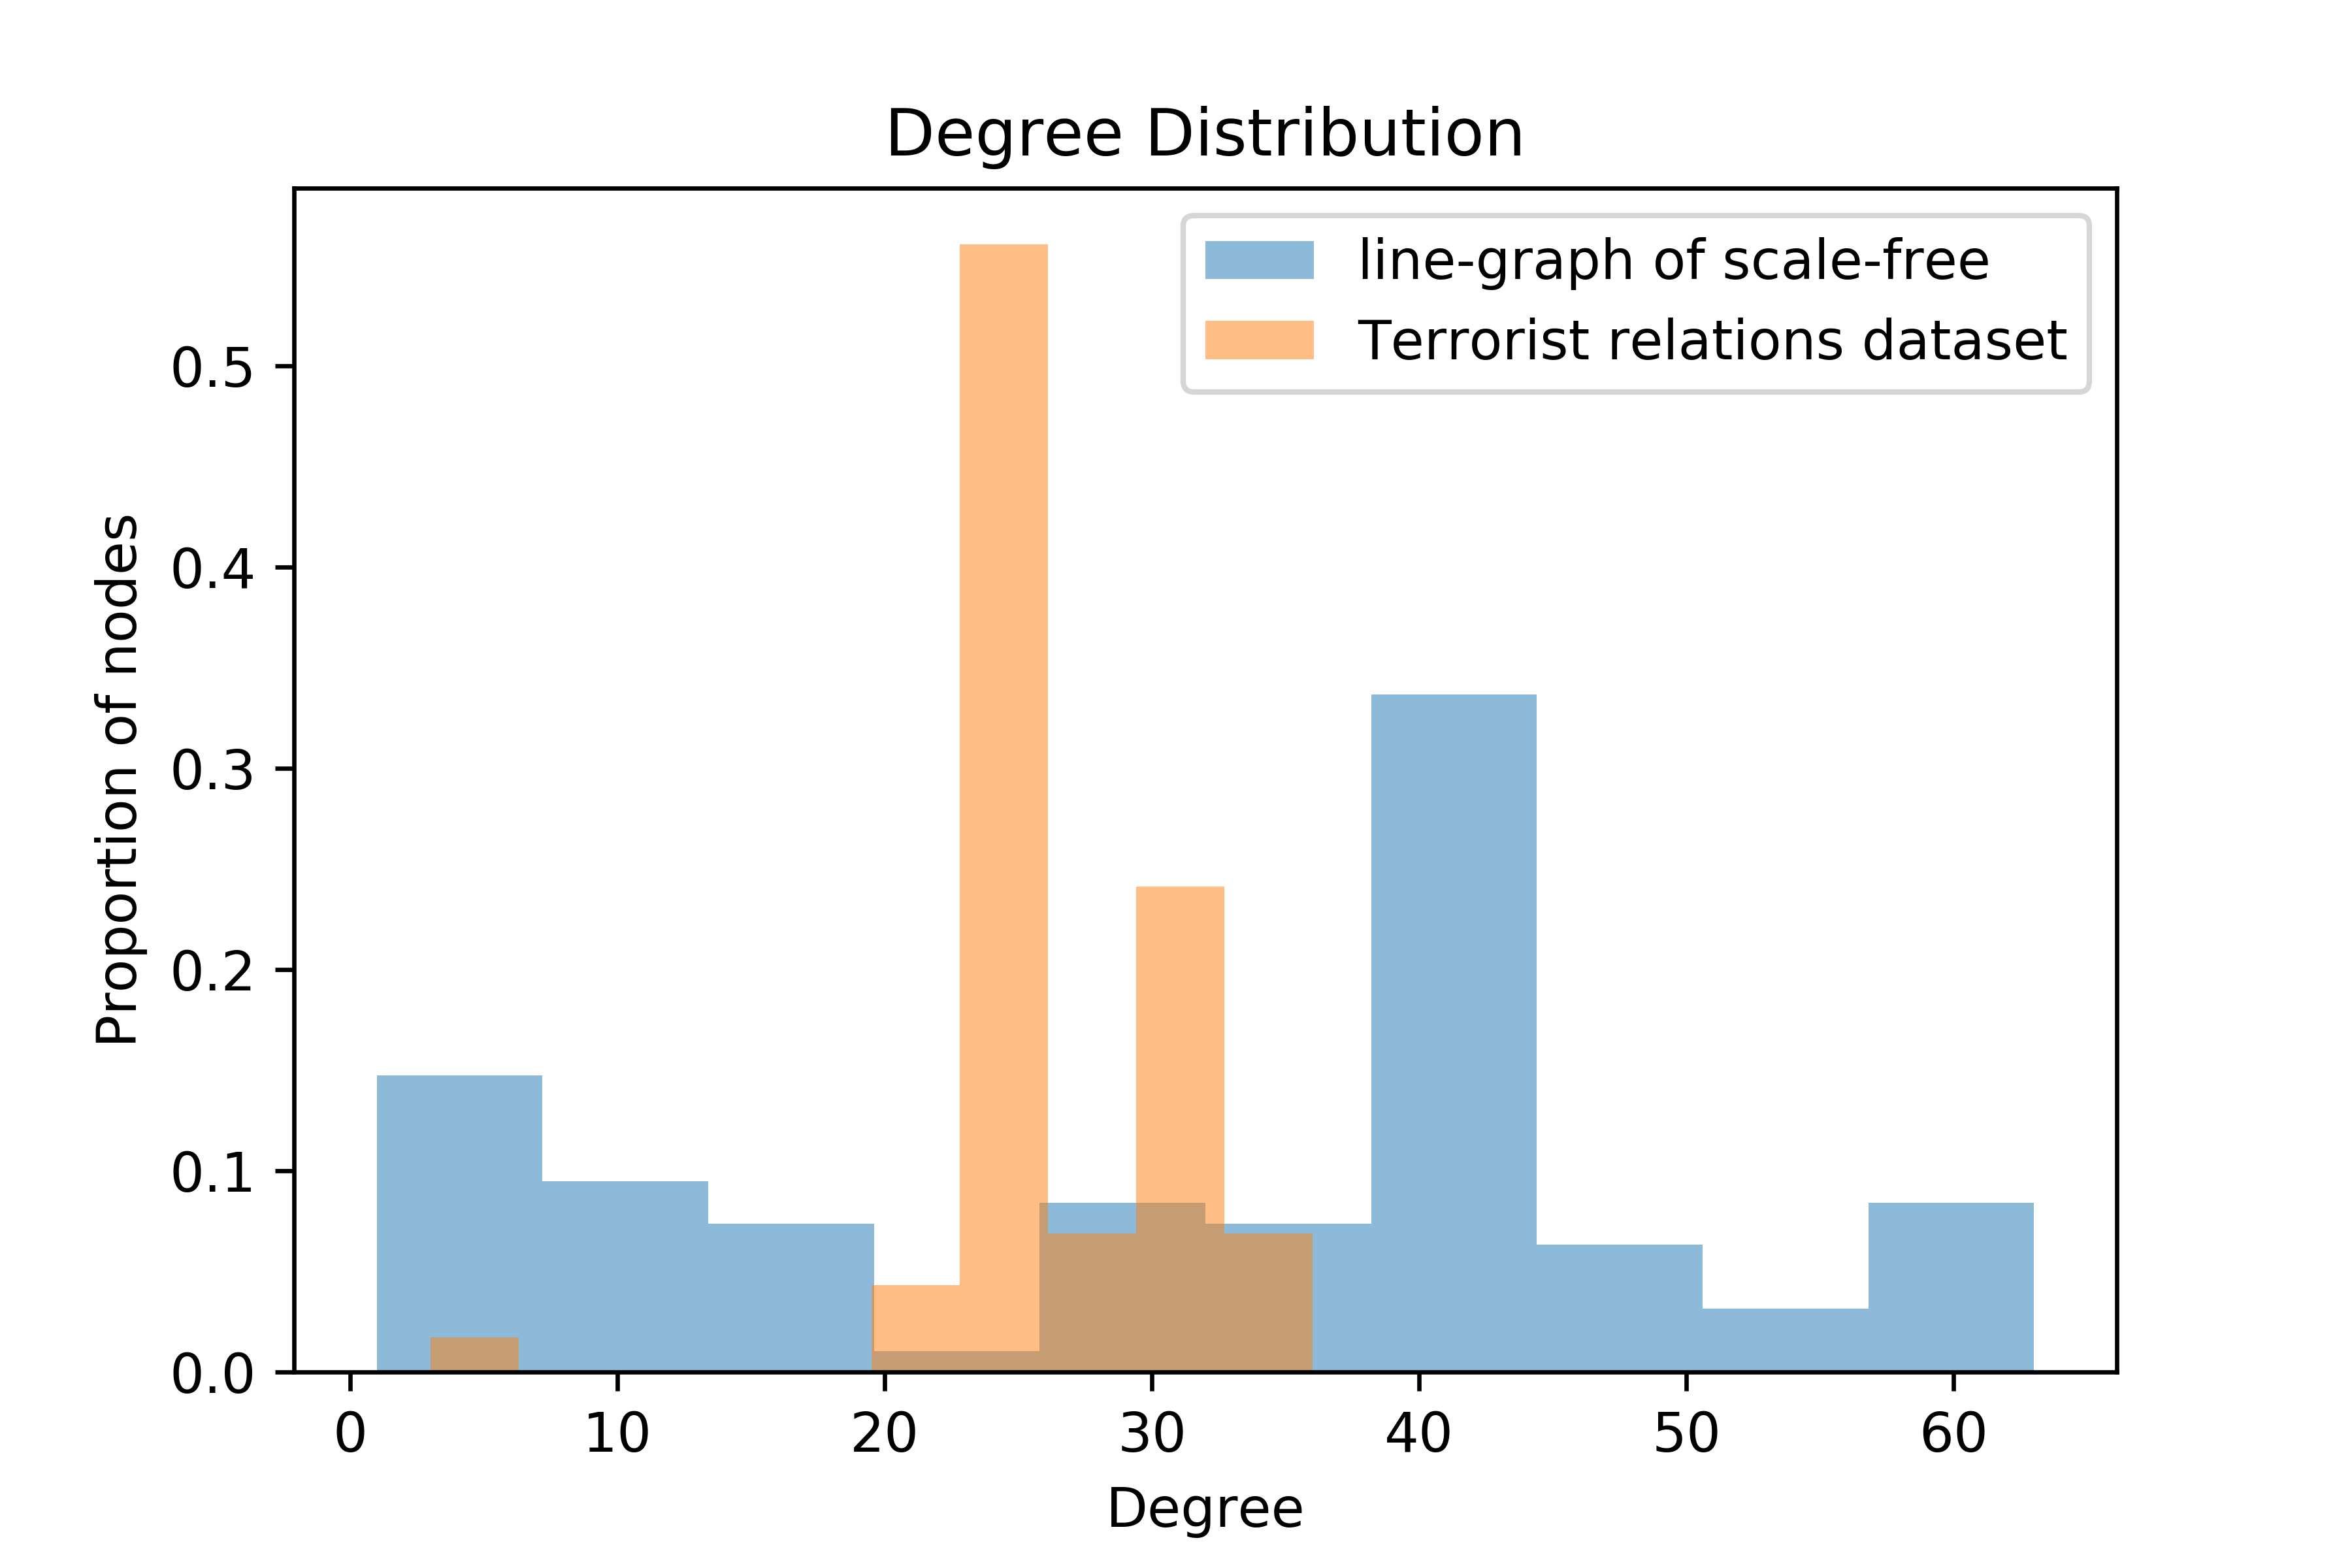
\includegraphics[width=.5\textwidth]{DegreeDiff.png}
\caption{Difference in degree between the dataset and the line graph}
\label{fig:degdiff}
\end{center}
\end{figure}
\end{frame}

% ----------------------------------------------------------------------------------------